%%%%%%%%%%%%%%%%%%%%%%%%%%%%%%%%%%%%%%%%%%%%%%%%%%
%%%%		~~~~ Method ~~~~
%%%%%%%%%%%%%%%%%%%%%%%%%%%%%%%%%%%%%%%%%%%%%%%%%%


\chapter{Éléments du calcul fractionnaire}
\label{chap:Dérivées et Intégrales d'ordre non entier}
\pagestyle{fancy}
\section{Intégrale fractionnaire au sens de Riemann-Liouville} 
\subsection{Définition}
L'approche de Riemann-Liouville offre une perspective solide et intuitive sur l'intégration fractionnaire. Cette méthode est basée sur la formule de Cauchy pour le n-ème intégral qui utilise seulement une simple intégration.
\begin{equation} \label{eq:int_succ}
    I_{a}^{n} f(t) = \int_{a}^{t} \int_{a}^{\tau_{n-1}} ... \int_{a}^{\tau_1} f(\tau) d\tau d\tau_1 ... d\tau_{n-1} = \frac{1}{(n-1)!}\int_{a}^{t} (t-\tau)^{n-1} f(\tau)d\tau
\end{equation}
\begin{proof}
    Par récurrence, le cas où $ n= 1$ est évidemment vérifié. Ainsi, nous allons montrer le cas où $n=2$.
    On a 
    \begin{align*}
    \frac{1}{1!} \int_{a}^{t} (t - \tau) f(\tau) d\tau &= \left|^{u = t-\tau}_{v'= f(\tau)} \hspace{0.5cm} {_{v = \int_{a}^{\tau} f(r) dr} ^{u'=-1}}\right| \\
    &= \left[(t-\tau)\int_{a}^{\tau}f(r)dr \right]_{\tau=a}^{\tau=t} + \int_{a}^{t}\int_{a}^{\tau}f(r)dr = {}_{a}I_t^2 f(t)
    \end{align*}
    
    En effet, à la limite supérieure, le polynôme est nul, tandis qu'à la limite inférieure, nous intégrons sur un ensemble de mesure nulle.\\
    Nous supposons maintenant que la formule est valide pour $n$ général. Nous procédons alors à une intégration supplémentaire $n+1$
    \begin{align*}
        \int_{a}^{t} I_{a}^{n} f(r)dr &= \int_{a}^{t}  \frac{1}{(n-1)!} \int_{a}^{r} (r - \tau)^{n-1} f(\tau) d\tau dr \\
        &= \frac{1}{(n-1)!} \int_{a}^{t}f(\tau)\int_{\tau}^{t} (r - \tau)^{n-1} drd\tau
        = \frac{1}{(n-1)!} \int_{a}^{t}f(\tau) \left[ \frac{(r-\tau)^n}{n} \right]_\tau ^t d\tau \\
        &= \frac{1}{n!} \int_{a}^{t} (t-\tau)^n f(\tau) d\tau \\
        &= I_a^{n+1} f(t)
    \end{align*}
\end{proof}
Puisque la fonction Gamma prolonge la fonction factorielle à l'ensemble des nombres réels, nous pouvons remplacer l'entier $n$ par le nombre réel positif $\alpha$, dans \ref{eq:int_succ}, alors nous obtenons la définition suivante:
\begin{definition}
    L'intégrale fractionnaire de Riemann-Liouville d'ordre $\alpha \in \mathbb{R^+}$ d'une fonction $f\in \textbf{L}^1 [a,b]$ est définie par:
    \begin{equation}\label{eq:integraleR-L}
        I_{a}^{\alpha} f(t) = {}_a^{RL} D_t^{-\alpha} f(t) =\frac{1}{\Gamma(\alpha)} \int_{a}^{t} (t-s)^{\alpha-1} f(s) ds.
    \end{equation}
\end{definition}
L'intégrale fractionnaire $I_a^{\alpha} f$ peut être réécrite sous la forme :
\begin{equation}
    I_{a}^{\alpha} f(t) = \frac{1}{\Gamma(\alpha)} \int_{0}^{t-a} s^{\alpha -1}f(t-s)ds, \hspace{1cm} t\in[a,b].
\end{equation}
Nous aboutissons donc au théorème suivant:
\begin{theoreme}
    Soient $f\in \textbf{L}^1 [a,b]$ et $\alpha > 0$. Alors, l'intégrale fractionnaire $I_a^{\alpha}$ existe pour tout $t\in[a,b]$ et la fonction $I_a^{\alpha} f$ est un élément de $\textbf{L}^1 [a,b]$. 
\end{theoreme}
\subsection{Intégrales fractionnaires au sens de R-L de quelques fonctions usuelles}
\subsubsection*{Fonction puissance} 
Soit la fonction $f(t)=(t-a)^\beta$, \hspace{0.3cm} $t\in[a,b]$, \hspace{0.3cm} $a\in\mathbb{R}$ \hspace{0.3cm} et $\beta > -1$. \\
Par la relation \ref{eq:integraleR-L} on a:
\begin{equation*}
    I_{a}^{\alpha} (t-a)^\beta=\frac{1}{\Gamma(\alpha)} \int_{a}^{t}(t-s)^{\alpha - 1} (s-a)^{\beta}ds
\end{equation*}
    et par le changement de variable $\tau = a + (t-a)s$, on obtient
    \begin{align*}
         I_{a}^{\alpha} (t-a)^{\beta} &= \frac{(t-a)^{\beta+\alpha}}{\Gamma(\alpha)} \int_0^1 s^{\beta - 1 + 1}(1-s)^{\alpha - 1}\\
         &= \frac{(t-a)^{\beta + \alpha}}{\Gamma(\alpha)} B(\alpha, \beta +1)\\
         &= \frac{(t-a)^{\beta + \alpha}}{\Gamma(\alpha)} \frac{\Gamma(\alpha)\Gamma(\beta + 1)}{\Gamma(\beta + \alpha + 1)}
\end{align*}
alors  l'intégral fractionnaire au sens de Riemann-Liouville de $f$ est donné par
\begin{equation} \label{eq:I_R-L_fct_puissance}
    I_{a}^{\alpha} (t-a)^\beta=\frac{\Gamma(\beta +1)}{\Gamma(\beta + \alpha + 1)}(t-a)^{\beta + \alpha}.
    \end{equation}

\begin{exemple}
En particulier, de \ref{eq:I_R-L_fct_puissance} si $a=0$, on a
\begin{equation*}
    I_{0}^{\alpha} (t)^{\beta} = \frac{\Gamma(\beta + 1)}{\Gamma(\beta + \alpha + 1)}t^{\beta + \alpha}
\end{equation*}
    et si $\alpha = \frac{1}{2}$ et $a = 0$, on a 
    \begin{enumerate}
        \item $I_0^{\frac{1}{2}}t^0=\frac{\Gamma(1)}{\Gamma(\frac{3}{2})} t^{\frac{1}{2}} = 2\sqrt{\frac{t}{\pi}}$
        \item $I_0^{\frac{1}{2}} t^1=\frac{\Gamma(2)}{\Gamma(\frac{5}{2})} t^{\frac{3}{2}} = \frac{4}{3}\sqrt{\frac{t^3}{\pi}}$
        \item $I_0^{\frac{1}{2}} t^2  =\frac{\Gamma(3)}{\Gamma(\frac{7}{2})} t^{\frac{5}{2}} = \frac{16}{15}\sqrt{\frac{t^5}{\pi}}$
    \end{enumerate}
\end{exemple}
\subsubsection*{Fonction constante} 
Soit $f(t) =C \in \mathbb{R}$ est une constante. Alors 
\begin{equation} \label{integral_R-L}
    I_{a}^{\alpha} C= \frac{C}{\Gamma(\alpha + 1)}(t-a)^\alpha
\end{equation}
\begin{exemple}
    Soit $f$ la fonction définie sur $\mathbb{R}$ par : $f(t) = 1$\\
    \begin{equation*}
        I_a^{\alpha}(1) = \frac{(t-a)^\alpha}{\Gamma(\alpha + 1)}
    \end{equation*}
\end{exemple}
\subsubsection*{Fonction exponentielle} Soit $f(t) = e^{kt}$, où $k\in \mathbb{R}$ est une constante, alors par la \ref{eq:I_R-L_fct_puissance} on a :
\begin{equation*}
     I_{a}^{\alpha} e^{kt}=\frac{1}{\Gamma(\alpha)} \int_{a}^{t} (t-s)^{\alpha - 1}e^{ks}ds
\end{equation*}
En faisant le changement de variable $s=t-\tau$, on obtient
\begin{equation*}
    I_{a}^{\alpha} e^{kt}=\frac{1}{\Gamma(\alpha)} \int_{0}^{t-a} s^{\alpha - 1} e^{k(t-s)}ds
\end{equation*}
Alors l'intégrale fractionnaire au sens de Riemann-Liouville de $f$ est donnée par:
\begin{equation}\label{eq:I_R-L_f_expo}
    I_{a}^{\alpha} e^{kt}=\frac{1}{\Gamma(\alpha)} \int_{0}^{t-a} s^{\alpha - 1}e^{k(t-s)} ds.
\end{equation}
\subsection{Quelques propriétés de base}
    La formule \ref{eq:integraleR-L} représente l'intégrale d'ordre arbitraire $\alpha > 0$, mais ne permet pas l'ordre $\alpha = 0$ qui correspond formellement à l'opérateur d'identité. \\
    Si la fonction $f$ est continue pour $t \geq a$, alors on considère la limite : $\lim_{\alpha\to 0^+} (I_{a}^{\alpha}f)(t) = f(t)$ \cite{FDEs_intro}.\\
    par conséquent nous pouvons écrire $I_a^0 f(t)=f(t)$ \\
\heading{Composition des intégrales fractionnaires}
L'opérateur intégral fractionnaire de Riemann-Liouville vérifie la propriété suivante:
\begin{proposition}
    Soient $f \in C[a,b]$ $\beta >0$, et $\alpha >0$. Alors on a 
    \begin{equation}
        I_{a}^{\alpha}[I_{a}^{\beta}f(t)] = I_{a}^{\alpha + \beta} f(t)
    \end{equation}
\end{proposition}
\begin{proof}
La preuve découle directement de la définition \ref{eq:integraleR-L}:
    \begin{align*}
        I_a^{\alpha}[I_a^{\beta}f(t)] &= I_a^{\alpha}[\frac{1}{\Gamma(\beta)} \int_{a}^{t} (t-s)^{\beta-1} f(s) ds] = I_a^{\alpha}[g(s)ds]\\
        &= \frac{1}{\Gamma(\alpha)} \int_{a}^{\tau} (\tau - u)^{\alpha - 1} [g(u) du] \\
        &= \frac{1}{\Gamma(\alpha)} \int_{a}^{\tau} (\tau - u)^{\alpha - 1} \left[\frac{1}{\Gamma(\beta)} \int _{a}^{t} (t-u)^{\beta - 1} f(u)du\right] \\
        &= \frac{1}{\Gamma(\alpha) \Gamma(\beta)} \int_{a}^{\tau} (\tau - t) \int_{a}^{t}(t-u)^{\beta - 1} f(u)du\\
    \end{align*}
    et par le changement de variable $ t = u + (\tau - u)$ on obtient:\\
    \begin{align*}
        I_{a}^{\alpha}[I_{a}^{\beta}f(t)] = \frac{\beta(\alpha, \beta)}{\Gamma(\alpha) \Gamma(\beta)} \int_{a}^{\tau} (\tau - t)^{\alpha + \beta - 1} f(u) du = I_{a}^{\alpha + \beta} f(t)
    \end{align*}
\end{proof}

\begin{proposition}
    Pout tout $\alpha, \beta >0$ et $f$ Lebesgue-intégrable sur $[a,b]$ on a :
    \begin{equation}
        \frac{d^k}{dt^k}[I_a^{\alpha} f(t)] = I_{a}^{\alpha - k} f(t) , \alpha >1, \hspace{1cm}\forall k <\alpha.
    \end{equation}
\end{proposition}
\begin{remarque}
    En générale: $D[_{a}I_t^{\alpha}f(t)] \neq {}_{a}I_t^{\alpha} [D f(t)]$ et alors on a le théorème suivant:
\end{remarque}
\begin{theoreme}
    Soient $f$ fonction continue sure $[0,b[$. Si $Df$ est continue alors pour tout $t>0$ on a :
    \begin{equation}
        D[I_{t}^{\alpha}f(t)] = I_{t}^{\alpha}[Df(t)]+\frac{f(0)}{\Gamma(\alpha)}t^{n-\alpha}
    \end{equation}
\end{theoreme}

\section{Dérivée fractionnaire au sens de Riemann-Liouville}
\subsection{Définition}
Tout d'abord, rappelons que pour tout fonction $f$ ayant une dérivée d'ordre $n$ continue sur l'intervalle $[a,b]$, nous avons:
\begin{equation}\label{eq:def_R-L}
    D^n = D^m I^{m-n} f,
\end{equation}
où $n,m\in\mathbb{N}$, tel que $m>n$. \\
Supposons que $n$ n'est pas un entier. Nous arrivons à la définition de l'opérateur différentiel fractionnaire de Riemann-Liouville. Cependant, il n'existe pas d'équivalent pour la n-ème dérivée comparable à \ref{eq:int_succ}, ce qui nous oblige à généraliser les dérivées via une intégrale fractionnaire. Initialement, nous introduisons une perturbation de l'ordre entier à l'aide d'une intégrale fractionnaire selon \ref{integral_R-L}, puis nous employons un nombre approprié de dérivées conventionnelles. \cite{FDE&applications}
\begin{definition}
    La dérivée fractionnaire au sens de Riemann-Liouville d'ordre $\alpha$ de la fonction $f$, notée $ \textbf{D}_a^{\alpha}$, est la fonction définie par :\\
    \begin{equation} \label{eq:D_R-L}
        \textbf{D}_a^{\alpha} = \frac{d^n}{dt^n} \left[I_a^{n-\alpha} f(t) \right],
    \end{equation}
    avec $n =[\alpha] + 1$ où $[.]$ est la partie entière. 
\end{definition}
De manière équivalente, nous avons:
\begin{equation}
    \textbf{D}_a^{\alpha} =
    \begin{cases}
        \frac{1}{\Gamma(n-\alpha)} \frac{d^n}{dt^n}\left( \int_a^t(t-s)^{n-\alpha-1}f(s)ds\right) \hspace{1cm} n-1<\alpha<n, \hspace{0.3cm} n\in\mathbb{N^*}\\
        \frac{d^n}{dt^n} f(t), \hspace{1cm} \alpha =n.
    \end{cases}
\end{equation}
\subsection{Dérivées fractionnaires de quelques fonctions usuelles}
\subsubsection*{Fonction puissance} 
Soient la fonction $g(t)=(t-a)^\gamma$, et $0<n-1<\alpha<n$ avec $\gamma > n-1$ on a alors: 
\begin{equation*}
    \textbf{D}_a^{\alpha} (t-a)^{\gamma} = \frac{1}{\Gamma(n-\alpha)} \frac{d^n}{dt^n} \int_a^t(t-\tau)^{n-\alpha-1} (\tau -a)^{\gamma} d\tau
\end{equation*}
    et par le changement de variable $\tau = a + (t-a)s$, on obtient
    \begin{align*}
         \textbf{D}_a^{\alpha} (t-a)^{\gamma} &= \frac{1}{\Gamma(n- \alpha)} \frac{d^n}{dt^n} (t-a)^{n+\gamma-\alpha} \int_0^1 (1-s)^{n-\alpha -1} s^{\gamma}ds\\
         &= \frac{\Gamma(n+\gamma-\alpha+1)B(n-\alpha,\gamma+1)}{\Gamma(n-\alpha)\Gamma(\gamma-\alpha +1)}(t-a)^{\gamma-\alpha}\\
         &= \frac{\Gamma(n+\gamma-\alpha+1)\Gamma(n-\alpha)\Gamma(\gamma +1)}{\Gamma(\gamma-\alpha +1)\Gamma(n-\alpha)\Gamma(n+\gamma-\alpha+1)}(t-a)^{\gamma-\alpha}\\
         &= \frac{\Gamma(\gamma+1)}{\Gamma(\gamma - \alpha +1)}(t-a)^{\gamma - \alpha}
\end{align*}
\begin{exemple}
Pour $\alpha = \frac{1}{2}, \gamma=\frac{1}{2}, a= 0$, nous aurons
\begin{equation*}
    \textbf{D}_a^{\frac{1}{2}} t^{\frac{1}{2}} = \frac{\Gamma(\frac{3}{2})}{\Gamma(1)}= \Gamma(\frac{3}{2}) 
\end{equation*}
\end{exemple}
\subsubsection*{Fonction constante} 
Soit $g(t) =C \in \mathbb{R}$ est une constante. Alors 
\begin{equation}
    \textbf{D}_a^{\alpha} C=\frac{C}{\Gamma(1-\alpha)}(t-a)^{-\alpha}.
\end{equation}
\subsection{Quelques Propriétés de base} 



\heading{Linéarité}

Soient $\lambda, \gamma\in \mathbb{R}$. D'après la définition de la dérivée fractionnaire de Riemann-Liouville, il vient que:
\begin{equation}
    \textbf{D}_a^{\alpha}(\lambda f(t) + \gamma g(t)) = \lambda\textbf{D}_a^{\alpha} f(t) +\gamma\textbf{D}_a^{\alpha} g(t).
\end{equation}
En effet,
\begin{align*}
    \textbf{D}_a^{\alpha}(\lambda f(t) + \gamma g(t)) &=  \frac{1}{\Gamma(n-\alpha)} \frac{d^n}{dt^n}\int_a^t (t-s)^{n-\alpha-1}(\lambda f(s)+\gamma g(s))ds\\
    &= \frac{\lambda}{\Gamma(n-\alpha)} \frac{d^n}{dt^n}\int_a^t(t-s)^{n-\alpha-1}f(s) ds +\frac{\gamma}{\Gamma(n-\alpha)} \frac{d^n}{dt^n}\int_a^t(t-s)^{n-\alpha-1}g(s)ds\\
    &=\lambda \textbf{D}_a^{\alpha} f(t) +\gamma\textbf{D}_a^{\alpha} g(t).
\end{align*}
\heading{Composition à droite avec intégrale fractionnaire}
Pour $\alpha>0$ et $t>a$, nous avons :
\begin{equation}
    \textbf{D}_a^{\alpha}\left(I_a^{\alpha}f(t)\right) = f(t)
\end{equation}
C'est-à-dire que l'opérateur de dérivation fractionnaire au sens de Riemann-Liouville est un inverse gauche de l'opérateur d'intégration fractionnaire
\begin{itemize}
    \item Cas où $\alpha=k\in\mathbb{N^*}$:\\
    \begin{align*}
        \textbf{D}_a^{\alpha}\left(I_a^{\alpha}f(t)\right) &= \frac{1}{\Gamma(n)}\frac{d^k}{dt^k}\int_a^t (t-a)^{k-1} f(s) ds\\
        &=\frac{d}{dt}\int_a^tf(s)ds\\
        &=f(t)
    \end{align*}
    \item Cas où $n-1\leq \alpha<n,  n\in\mathbb{N^*}$:\\
    Nous savons que :
    \begin{equation*}
        \left(I_a^{n-\alpha}(I_a^{\alpha}f(t)) \right) = I_a^nf(t)
    \end{equation*}
    et que :
    \begin{equation*}
         \textbf{D}_a^{\alpha}f(t) =  \frac{d^n}{dt^n} \left(I_a^{n-\alpha} f(t)\right)
    \end{equation*}
    Nous avons alors:
    \begin{align*}
        \textbf{D}_a^{\alpha}\left(I_a^{\alpha} f(t)\right) &= \frac{d^n}{dt^n} \left(I_a^{n-\alpha}(I_a^{\alpha}) f(t)\right)\\
        &= \frac{d^n}{dt^n}I_a^nf(t)\\
        &= f(t).
    \end{align*}
\end{itemize}
\heading{Composition à droite avec intégrale fractionnaire d'ordre différent}
Pour $\alpha \geq 0$ et $\beta \geq 0$, nous avons
\begin{equation*}
    \textbf{D}_a^{\alpha}\left(I_a^{\beta} f(t)\right) = \textbf{D}_a^{\alpha - \beta} f(t)
\end{equation*}
où $f$ est une fonction continue et que $\textbf{D}_a^{\alpha-\beta}f$ existe si $\alpha \geq \beta$.\\
Si $\alpha - \beta<0$, alors:
\begin{equation}
    \textbf{D}_a^{\alpha - \beta} f(t) = I_a^{\beta-\alpha}f(t).
\end{equation}
En effet,
\begin{itemize}
    \item Si $\beta \geq \alpha \geq 0$, nous avons :
    \begin{align*}
        \textbf{D}_a^{\alpha}\left(I_a^{\beta} f(t)\right) &= \textbf{D}_a^{\alpha}\left(I_a^{\alpha} I_a^{\beta-\alpha} f(t)\right)\\
        &= I_a^{\alpha - \beta} f(t)
    \end{align*}
    \item Si $\alpha>\beta\geq0$, nous avons:\\
    Pour $n$ et $m$ deux entiers tels que : $0\leq n-1 \leq \alpha < n$ et $0\leq m-1\leq\alpha - \beta<m$,
    \begin{align*}
        \textbf{D}_a^{\alpha}\left(I_a^{\beta} f(t)\right) &= \frac{d^n}{dt^n}\left(I_a^{n-\alpha}\left(I_a^{\beta} f(t)\right)\right)\\
        &= \frac{d^n}{dt^n}\left(I_a^{n-\alpha+\beta} f(t)\right)\\
        &= \frac{d^m}{dt^m}\left(I_a^{m-\alpha+\beta} f(t)\right)\\
        &= \textbf{D}_a^{\alpha - \beta} f(t)
    \end{align*}
\end{itemize}
\begin{remarque}
    Dans le cas des dérivées fractionnaires, la loi de composition ne peut pas être généralisée sans imposer des restrictions supplémentaires sur $f$. Elle n'est pas nécessairement vérifiée pour tout $\alpha$ et $\beta$. Nous allons énoncer précisément les conditions dans lesquelles cette loi s'applique.
\end{remarque}
\heading{Composition avec les dérivées d'ordre entier}
La composition de la dérivée fractionnaire de Riemann-Liouville avec la dérivée d'ordre entier apparaît dans de nombreux problèmes appliqués, il et donc pratique de l'introduire ici.\\
Pour $n \leq n-1 \leq \alpha < n$, $n\in \mathbb{N^*}$,
\begin{equation}
    \frac{d^k}{dt^k} \left( \textbf{D}_a^{\alpha} f(t) \right) = \textbf{D}_a^{k+\alpha} f(t),
\end{equation}
\begin{equation}\label{eq:composition_d_n}
    \textbf{D}_a^{\alpha}\left(\frac{d^k}{dt^k}f(t) \right)=\textbf{D}_a^{k+\alpha}f(t) - \sum _{i=1}^{k-1}\frac{f^{(i)}(a) (t-a)^{i-\alpha -k}}{\Gamma(i-\alpha-k+1)}.
\end{equation}
En effet, d'après la relation \ref{eq:D_R-L}, nous avons:
\begin{align*}
    \frac{d^k}{dt^k} \left( \textbf{D}_a^{\alpha} f(t) \right) &= \frac{1}{\Gamma(n-\alpha)} \frac{d^{n+k}}{dt^{n+k}} \int_a^t (t-s)^{n-\alpha-1} f(s)ds,\\
    &= \frac{1}{\Gamma((n+k)-(\alpha +k))} \frac{d^{n+k}}{dt^{n+k}}\int _a^t (t-s)^{(n+k)-(\alpha +k)-1}f(s)ds\\
    &= \textbf{D}_a^{k+\alpha} f(t),
\end{align*}
avec $(n+k-1\leq \alpha + k <n+k)$.
Pour l'égalité \ref{eq:composition_d_n}, nous avons d'après la formule \ref{eq:int_succ}:
\begin{align*}
    I_a^k f^{(k)} &= \frac{1}{(k-1)!}\int_a^t (t-s)^{k-1} f^{(k)} (s) ds,\\
    &= f(t) -\sum_{i=1}^{k-1} \frac{f^{(i)} (a) (t-a)^i}{\Gamma(i+1)}.
\end{align*}
Par conséquent, 
\begin{align*}
    \textbf{D}_a^{\alpha} \left(\frac{d^k}{dt^k}f(t) \right) = \textbf{D}_a^{\alpha}\left(f^{(k)}(t) \right),\\
    &= \textbf{D}_a^{\alpha+k} \left(I_a^k f^{(k)}(t) \right),\\
    &= \textbf{D}_a^{\alpha +k} \left(f(t) -\sum_{i=1}^{k-1} \frac{f^{(i)}(a)(t-a)^i}{\Gamma(i+1)} \right),\\
    &= \textbf{D}_a^{\alpha +k} f(t) -\sum_{i=1}^{k-1} \frac{f^{(i)}(a)(t-a)^{i-\alpha-n}}{\Gamma(i-\alpha -n +1)}.\\
\end{align*}
\heading{Composition avec les dérivées fractionnaires}
Pour $n-1\leq \alpha <n$ et $m-1\leq \beta <m$, nous avons:
\begin{equation}
    \textbf{D}_a^{\alpha} \left(\textbf{D}_a^{\beta} f(t) \right) = \mathbf{D}_a^{\alpha+\beta}f(t) -\sum_{i=1}^m [\textbf{D}_a^{\beta -i} f(t)]_t=a \frac{(t-a)^{-\alpha-i}}{\Gamma(-\alpha -i +1)},
\end{equation}
et
\begin{equation}
        \textbf{D}_a^{\beta} \left(\textbf{D}_a^{\alpha} f(t) \right) = \mathbf{D}_a^{\beta+\alpha}f(t) -\sum_{i=1}^n [\textbf{D}_a^{\alpha -i} f(t)]_{t=a} \frac{(t-a)^{-\beta-i}}{\Gamma(-\beta -i +1)},
\end{equation}
En effet, d'après la relation \ref{eq:def_R-L}, nous avons:
\begin{equation*}
    \textbf{D}_a^{\alpha} \left(\textbf{D}_a^{\beta} f(t)\right) = \frac{d^n}{dt^n} \left(I^{n-\alpha}(\textbf{D}_a^{\beta} f(t))\right)
\end{equation*}
Donc, nous aurons:
\begin{equation*}
    \textbf{D}_a^{\alpha}(\textbf{D}_a^{\beta} f(t)) = \frac{d^n}{dt^n} \left(\textbf{D}_a^{\alpha+\beta-n} f(t) -\sum_{i=1}^m [\textbf{D}_a^{\beta -i} f(t)]_ {t=a} \right) = \frac{(t-a)^{n-\alpha-i}}{\Gamma(n-\alpha-i+1)},
\end{equation*}
par la suite, nous avons:
\begin{equation*}
    \textbf{D}_a^{\alpha}(\textbf{D}_a^{\beta} f(t))=\textbf{D}_a^{\alpha+\beta} f(t) -\sum_{i=1}^m[\textbf{D}_a^{\beta-i}f(t)]_{t=a} \frac{(t-a)^{-\alpha-i}}{\Gamma(-\alpha-i+1)},
\end{equation*}
De meme pour:
\begin{equation*}
    \textbf{D}_a^{\beta}(\textbf{D}_a^{\alpha} f(t)) = \textbf{D}_a^{\beta+\alpha} f(t) -\sum_{i=1}^n[\textbf{D}_a^{\alpha-i}f(t)]_{t=a} \frac{(t-a)^{-\beta-i}}{\Gamma(-\beta -i+1)}.
\end{equation*}
En général, les opérateurs de dérivation fractionnaire, au sens de Riemann-Liouville, ne commutent pas. Mais, nous avons la propriété essentielle suivante:
\begin{equation}
    \textbf{D}_a^{\alpha}\left(\textbf{D}_a^{\beta} f(t)\right) = \textbf{D}_a^{\beta} \left( \textbf{D}_a^{\alpha} f(t)\right) = \textbf{D}_a^{\alpha+\beta}f(t),
\end{equation}
si et seulement si: \\
\begin{equation}
    \begin{cases}
        \textbf{D}_a^{\alpha -i} f(t)|_{t=a} =0, \hspace{1cm} i=1,2,...,n,\\
        \textbf{D}_a^{\beta -j} f(t)|_{t=a}=0, \hspace{1cm} j=1,2,...,m.
    \end{cases}    
\end{equation}
\section{Dérivée fractionnaire au sens de Caputo}
Avant de présenter la définition, il est important de souligner les similitudes structurelles avec la dérivée de Riemann-Liouville. Tout comme la dérivée de Riemann-Liouville utilise une intégrale fractionnaire pour capturer les comportements passés d'une fonction, la dérivée de Caputo utilise également une intégrale fractionnaire pour prendre en compte les valeurs passées. Cependant, la différence majeure réside dans l'ordre de différentiation, où la dérivée de Caputo permet d'effectuer une dérivation d'ordre non entier. Cette approche conduit à la définition suivante de la différentielle de Caputo. \cite{FDE&applications}

\begin{definition}
    La dérivée fractionnaire de Caputo est définie par:
    \begin{equation}\label{eq:der_frac_caputo}
        D_a^{alpha} f(t) = I_a^{m-\alpha}\left(\frac{d^m}{dt^m} f(t) \right) = \frac{1}{\Gamma(m-\alpha)}\int_a^t (t-\tau)^{m-\alpha -1} f^{(m)} (s)ds,
    \end{equation}
    pour $m-1\leq\alpha<m$, $m\in \mathbb{N}$, $t>a$
\end{definition}
$m$ est utilisé dans la définition de la dérivée de Caputo plutôt que $n$ utilisé dans la dérivée de Riemann-Liouville afin d'assurer la correspondance avec les dérivées d'ordre entier. 
Si nous utilisions $n$ dans la définition de Caputo, cela donnerait des résultats erronés pour la k-ème dérivée d'une fonction ayant une $(k + 1)$-ème dérivée nulle. Cela entraînerait un paradoxe où nous aurions besoin d'une fonction $(k + 1)$-fois différentiable pour obtenir la k-ème dérivée. En utilisant $m$ dans la dérivée de Riemann-Liouville, nous pourrions éviter ce problème, mais nous utilisons $n$ car cela ne nécessite pas de relation limite. En résumé, la différence entre $n$ et $m$ n'est présente que pour les entiers, et les deux cas se rejoignent aux points correspondant aux dérivées classiques. Cela garantit une cohérence entre les dérivées fractionnaires et les dérivées d'ordre entier, sans aucun problème.

%% plots
{
\centering
\begin{minipage}[t]{.5\textwidth}
    \begin{flushleft}
        \resizebox{\textwidth}{!}{
        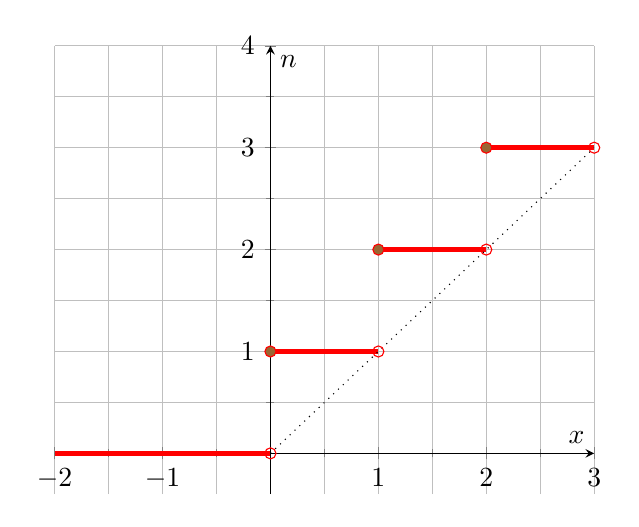
\begin{tikzpicture}
            \begin{axis}[ 
                xlabel=$x$, ylabel={$n$}, 
                axis lines=middle, 
                domain=-2:3, 
                samples=400, 
                ytick={-1,0,1,2,3, 4},
                unbounded coords=jump, % treat jumps in the function as discontinuities
                grid=both,
                minor tick num = 1,
                enlarge y limits={value=0.1,lower}
                ]
                \addplot+[red, no markers, ultra thick, samples at={-2,...,3}, jump mark left] {{ifthenelse(x<0,0,ceil(x) + 1)}}; 
                \addplot+[red, only marks, mark=o, samples at={0,...,3}] {ceil(x)}; 
                \addplot+[red, only marks, mark=*, samples at={0,...,2}] {ceil(x) + 1};
                \addplot[black, dotted, domain=0:3] {x};
            \end{axis}
        \end{tikzpicture}
        }%
        \captionof{figure}{La fonction $n = [\alpha] + 1$ utilisée pour la dérivée de Riemann-Liouville.}
        \label{fig:riemannliouville}
    \end{flushleft}
\end{minipage}%
\begin{minipage}[t]{.5\textwidth}
    \begin{flushright}
        \resizebox{\textwidth}{!}{
        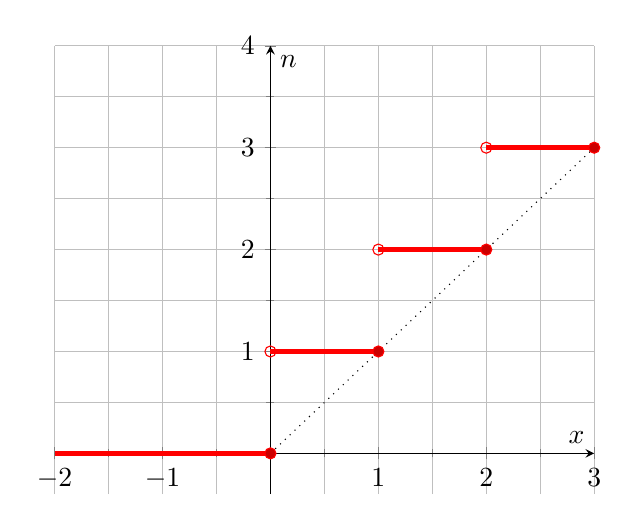
\begin{tikzpicture}
            \begin{axis}[
                xlabel=$x$, ylabel={$n$}, 
                axis lines=middle, 
                domain=-2:3, 
                samples=400, 
                ytick={-1,0,1,2,3, 4},
                unbounded coords=jump, % treat jumps in the function as discontinuities
                grid=both,
                minor tick num = 1,
                enlarge y limits={value=0.1,lower}
                ]
                \addplot+[red, no markers, ultra thick, samples at={-2,...,3}, jump mark left] {{ifthenelse(x<0,0,ceil(x) + 1)}}; 
                \addplot+[red, only marks, mark=*, samples at={0,...,3}] {ceil(x)}; 
                \addplot+[red, only marks, mark=o, samples at={0,...,2}] {ceil(x) + 1};
                \addplot[black, dotted, domain=0:3] {x};
            \end{axis}
        \end{tikzpicture}
        }%
        \captionof{figure}{La fonction $n = - [-\alpha]$ utilisée pour la dérivée de Caputo.}
        \label{fig:caputo}
    \end{flushright}
\end{minipage}
}
\vspace{0.5cm}
\begin{remarque}
    Si $\alpha \to m$, alors $D_a^{\alpha}f$ coïncide avec $\frac{d^m}{dt^m}$.
    En effet, supposons que la fonction $f$ admet $(m+1)$ dérivée bornées continues dans $[a,T]$ pour tout $T>a$. Alors
    \begin{align*}
        \lim_{\alpha\to m} D_a^{\alpha} f(t) &= \lim_{\alpha \to m} \left(\frac{f^{(m)}(a)(t-a)^{m-\alpha}}{\Gamma(m-\alpha+1)} +\frac{1}{\Gamma(m-\alpha + 1)}\int_a^t (t-s)^{m-\alpha-1} f^{(m+1)} (s)ds \right),\\
        &= f^{(m)}(a) +\int_a^t f^{(m+1)}(s)ds,\\
        &= f^{(m)} (t).
    \end{align*}
    Ainsi,
    \begin{align*}
        \lim_{\alpha \to m} D_a^{\alpha} f =\frac{d^m}{dt^m}f.
    \end{align*}
    L'avantage principale de la dérivée fractionnaire de Caputo es de conditions initiales des équations différentielles et aux dérivées partielles fractionnaires avec des dérivée au sens de Caputo acceptent la même forme comme pour les équations différentielles et aux dérivées partielles d'ordre entiers. C-à-d contient des valeurs limites des dérivées d'ordre entier des fonctions inconnues en la borne inférieure $t=a$.
\end{remarque}

\subsection{Dérivées fractionnaires de quelques fonctions usuelles}
\subsubsection*{Fonction puissance} 
Soit la fonction $g(t)=(t-a)^\gamma$,\\
Soient $ 0 < m-1 < \alpha < m$, avec $\gamma > m-1$, alors nous avons:\\
\begin{equation*}
    g^{(m)}= \frac{\Gamma(\gamma + 1)}{\Gamma(\gamma-m+1)}(t-a)^{\gamma-m},
\end{equation*}
d'où,
\begin{equation*}
    D_a^{\alpha}(t-a)^{\gamma} = \frac{\Gamma(\gamma +1)}{\Gamma(\gamma - m +1) \Gamma(m-\alpha)}\int_a^t(t-\tau)^{m-\alpha-1} (\tau -a)^{\gamma -m}d\tau.
\end{equation*}
    et par le changement de variable $\tau = a + (t-a)s$, on obtient :
    \begin{align*}
    D_a^{\alpha}(t-a)^{\gamma} &= \frac{\Gamma(\gamma +1)}{\Gamma(\gamma - m +1)\Gamma(m-\alpha)}(t-a)^{\gamma - \alpha} \int_a^1(1-s)^{m-\alpha-1} s^{\gamma-m}ds,\\
    &= \frac{\Gamma(\gamma+1)\beta(m-\alpha,\gamma-m+1)}{\Gamma(\gamma-m+1)\Gamma(m-\alpha)\Gamma(\gamma-\alpha+1)}(t-a)^{\gamma-\alpha},\\
    &= \frac{\Gamma(\gamma+1)\Gamma(m-\alpha)\Gamma(\gamma -m +1)}{\Gamma(\gamma-m +1)\Gamma(m-\alpha)\Gamma(\gamma-\alpha+1)}(t-a)^{\gamma-\alpha},\\
    &= \frac{\Gamma(\gamma +1)}{\Gamma(\gamma-\alpha+1)}(t-a)^{\gamma-\alpha}.
\end{align*}
Donc,
\begin{equation*}
    D_a^{\alpha}(t-a)^{\gamma} = \frac{\Gamma(\gamma+1)}{\Gamma(\gamma-\alpha+1)}(t-a)^{\gamma - \alpha}.
\end{equation*}
\begin{exemple}
Pour $a= 0$, la dérivée fractionnaire de Caputo d'ordre $\gamma$ de la fonction $g(t)^\gamma$ est donnée par :
\begin{equation*}
    {D}_a^{\alpha} t^{\gamma} =
    \begin{cases}
            \frac{\Gamma(\gamma +1)}{\Gamma(\gamma-\alpha+1)}t^{\gamma-\alpha}, \hspace{0.5cm} \gamma>\alpha-1,\\
            0, \hspace{2.51cm} \gamma \leq \alpha -1.
        \end{cases}
\end{equation*}
\end{exemple}


\subsubsection*{Fonction constante} 
Soit $g(t) =C \in \mathbb{R}$ est une constante. Alors 
\begin{align*}
    D_a^{\alpha} g(t) &= \frac{1}{\Gamma(m-\alpha)} \int_a^t (t-s)^{m-\alpha-1} g^{(m)}(s) ds,\\
    &= \frac{1}{\Gamma(m-\alpha)}\int_a^t(t-s)^{m-\alpha-1} \times 0ds \\
    &=0
\end{align*}
Par la suite
\begin{equation*}
    D_a^{\alpha} C = 0.
\end{equation*}
\subsection{Quelques propriétés de base}
\heading{Linéarité}
Soient $\lambda$, $\gamma \in \mathbb{R}$. D'après la définition de la dérivée fractionnaire de Caputo, il vient que :
\begin{equation}
    D_a^{\alpha}(\lambda f(t)+\gamma g(t))=\lambda D_a^{\alpha}f(t) + \gamma D_a^{\alpha}g(t).
\end{equation}
\heading{Relation avec la dérivée fractionnaire de Riemann-Liouville}
Pour $0\leq m-1<\alpha<m$ et $f$ une fonction telle que $D_a^{\alpha}$ et $\textbf{D}_a^{\alpha}$ existent. Alors 
\begin{equation}
    D_a^{\alpha} f(t) = \textbf{D}_a^{\alpha}f(t) -\sum_{k=0}^{m-1} \frac{f^{(k)}(a)(t-a)^{k-\alpha}}{\Gamma(k-\alpha+1)}.
\end{equation}
Par conséquent, si $f^{(k)}(a)=0$ pour $k=0,1,...,m-1$, alors la dérivée de Caputo coïncide avec celle de Riemann-Liouville pour tout $\alpha\in\mathbb{R}$, c'est à dire:
\begin{equation*}
    D_a^{\alpha} f(t) = \textbf{D}_a^{\alpha} f(t).
\end{equation*}
\heading{Composition avec l'opérateur d'intégration fractionnaire}
Si $f$ est continue, alors
\begin{equation*}
    D_a^{\alpha}(I_a^{\alpha})=f(t),
\end{equation*}
et \begin{equation*}
    I_a^{\alpha}\left(D_a^{\alpha} f(t) \right)=f(t)-\sum_{k=0}^{m-1} \frac{f^{(k}(a)(t-a)^k}{k!}.
\end{equation*}
Ainsi l'opérateur de dérivation de Caputo est un inverse gauche de l'opérateur d'intégration fractionnaire, mais il n'est pas un inverse droit.
\heading{Composition avec la dérivée d'ordre entier}
Soient $n\in\mathbb{N}$ et $m-1\leq\alpha<m$, alors:
\begin{equation}\label{eq:comp_o_n}
    D_a^{\alpha}(D_a^n f(t)) = d_a^{\alpha+n}f(t),
\end{equation}
et si $f^{(k)}(a)=0$ pour $k=0,1,..m-1$, nous avons:
\begin{equation}
    D_a^n\left( D_a^{\alpha} f(t) \right) = D_a^{N+\alpha} f(t).
\end{equation}
En effet, pour la relation \ref{eq:comp_o_n}, nous avons:
\begin{align*}
    D_a^{\alpha}(D_a^n f(t)) &= D_a^{-(m-\alpha)} D_a^m(D_a^n f(t)),\\
    &= D_a^{-(m-\alpha)} D_a^{m+n} f(t),\\
    &= D_a^{-(m+n-(\alpha +n)} D_a^{m+n} f(t)\\
    &= D_a^{\alpha + n} f(t)
\end{align*}
